%%
% The BIThesis Template for Bachelor Graduation Thesis
%
% 北京理工大学毕业设计开题报告 —— 使用 XeLaTeX 编译
%
% Copyright 2020-2021 BITNP
%
% This work may be distributed and/or modified under the
% conditions of the LaTeX Project Public License, either version 1.3
% of this license or (at your option) any later version.
% The latest version of this license is in
%   http://www.latex-project.org/lppl.txt
% and version 1.3 or later is part of all distributions of LaTeX
% version 2005/12/01 or later.
%
% This work has the LPPL maintenance status `maintained'.
%
% The Current Maintainer of this work is Feng Kaiyu.
%
% This work consists of the files main.tex, misc/cover.tex and
% the external PDF misc/reviewTable.pdf
%
% Compile with: xelatex -> biber -> xelatex -> xelatex

\documentclass[proposal-report]{bitart}

% 参考文献引用文件 refs.bib
\addbibresource{misc/refs.bib}

\newcommand{\deptName}{计算机学院}
\newcommand{\majorName}{计算机科学与技术}
\newcommand{\className}{07xxxxxx}
\newcommand{\yourName}{惠计算}
\newcommand{\mentorName}{张哈希}
\newcommand{\offCampusMentorName}{刘阿贝尔}

% 定义一个概念
\newtheorem{definition}{概念}[section]



%%
% 文档开始
\begin{document}
% 评审表
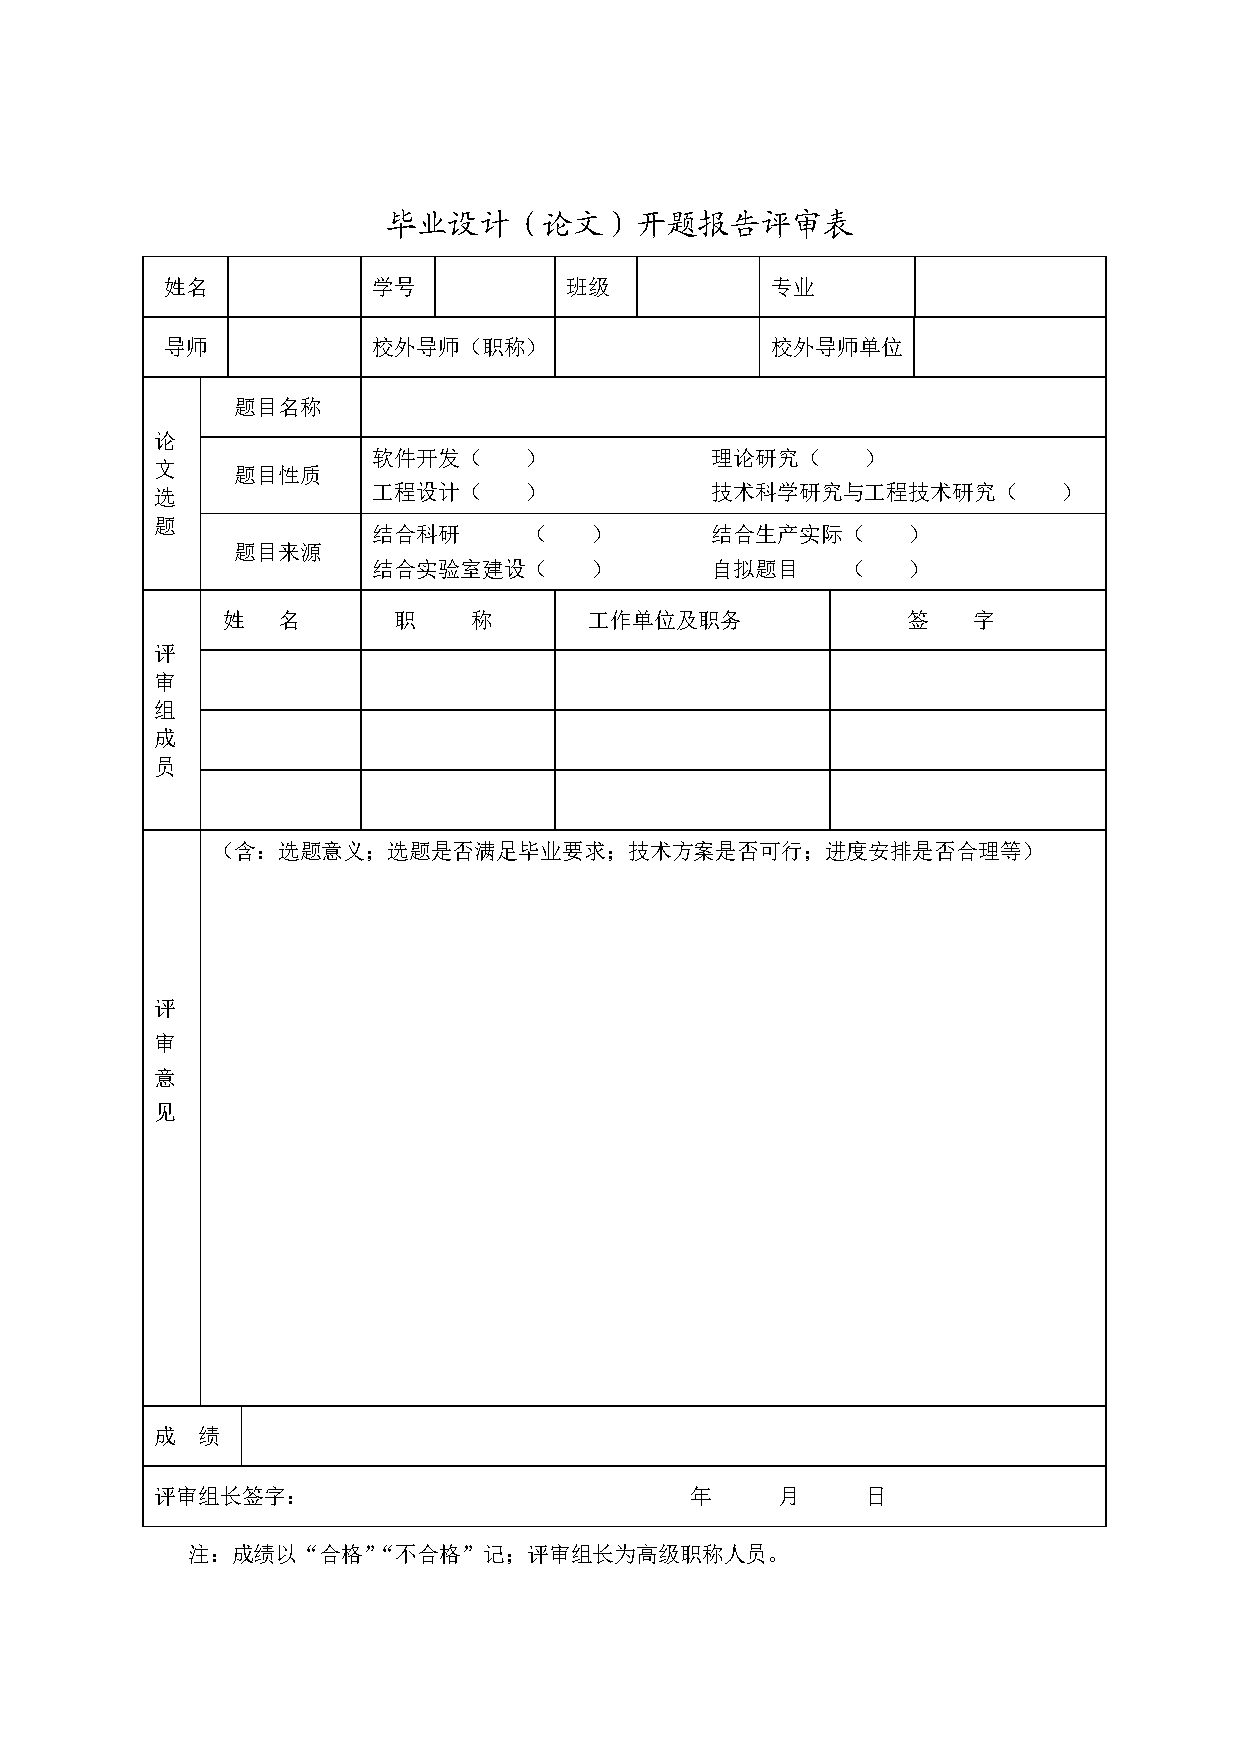
\includepdf[pages=-]{misc/reviewTableBlank.pdf}

%%
% 正文开始
\pagestyle{fancy}
% 正文从第一页开始计算页码
\setcounter{page}{1}


% 正文 22 磅的行距,段前段后间距为 0
\setlength{\parskip}{0em}
\renewcommand{\baselinestretch}{1.53}
% 正文首行悬挂 1.02cm
\setlength{\parindent}{1.02cm}

% 内容开始
\section{毕业设计(论文)选题的内容}
开题报告总长度约 5 至 6 页,本部分重点介绍毕业设计选题的主要内容 \cite{LeCun2010},宋体,小三,段落前后 0.5 行。

\section{研究方案}
\subsection{本选题的主要任务}
本部分重点关注毕业设计的主要任务,宋体,四号,段落前后 0.5 行。

\subsection{技术方案的分析、选择}
此部分要分析任务书,并给出初步方案,要体现出复杂系统的概念,约写 2 至 3 页。

\begin{figure}[!ht]
  \centering
  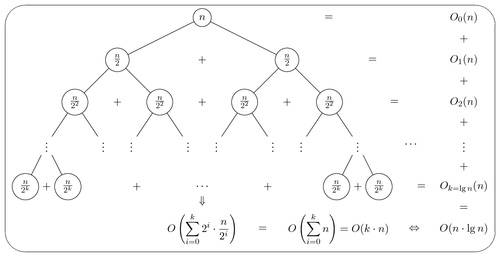
\includegraphics[width=0.6\linewidth]{merge-sort-recursion-tree}
  \caption{Merge sort recursion tree:一张示意图}
  \label{fig:mergesort}
\end{figure}

\subsubsection{第一阶段}
在第一阶段,我们准备……

\subsection{实施技术方案所需的条件}
此部分说明所需的软硬件等环境,建议使用表格的形式,方便表述。

\begin{table}[!ht]
  \centering
  \caption{硬件、软件环境}
  \label{tab:soft-hardware}
  \begin{tabular}{@{}lcl@{}}
    \toprule
                              & 指标     & \multicolumn{1}{c}{版本参数} \\ \midrule
    \multirow{2}{*}{硬件环境} & CPU      & Intel i7-6500U               \\ \cmidrule(l){2-3}
                              & RAM      & 8 GB                         \\ \midrule
    \multirow{2}{*}{软件环境} & 操作系统 & \begin{tabular}[c]{@{}l@{}}Windows 10 Pro x86\_64\\  Ubuntu 18.04.3 LTS\end{tabular}    \\ \cmidrule(l){2-3}
                              & Python   & Python 3.7.6                 \\ \bottomrule
  \end{tabular}
\end{table}

\subsection{存在的主要问题和技术关键}
目前存在的主要问题是……

正文,小四,行距 22 磅。

\subsection{预期能够达到的研究目标}
要包括最后提交的成果。

\section{课题计划进度表}
大致的课题计划进度如下表 \ref{tab:progress} 所示。

\begin{table}[!ht]
  \centering
  \caption{毕业设计计划进度表}
  \label{tab:progress}
  \begin{tabular}{@{}cllc@{}}
    \toprule
    阶段 & \multicolumn{1}{c}{任务} & \multicolumn{1}{c}{完成标志} & 时间规划       \\ \midrule
    1    & 第一阶段的任务……          & 成功搭建……                    & 2019.12-2020.1 \\ \midrule
    2    & 第二阶段的任务……          & 成功验证……                    & 2020.1-2020.2  \\ \midrule
    3    & 第三阶段的任务……          & 成功验证……失效,并优化……增强  & 2020.2-2020.4  \\ \midrule
    4    & 第四阶段的任务……          & 成功完成毕业设计              & 2020.4-2020.5  \\ \bottomrule
  \end{tabular}
\end{table}

注意:下文的参考文献应包含近 5 年内文献,经典文献除外。

\section{参考文献}
% 删除默认的「参考文献 / Reference」标题,使用上面定义的 section 标题
\printbibliography[heading=none]

\end{document}
